%
% kreis.tex
%
% (c) 2024 Prof Dr Andreas Müller
%
\begin{figure}
\centering
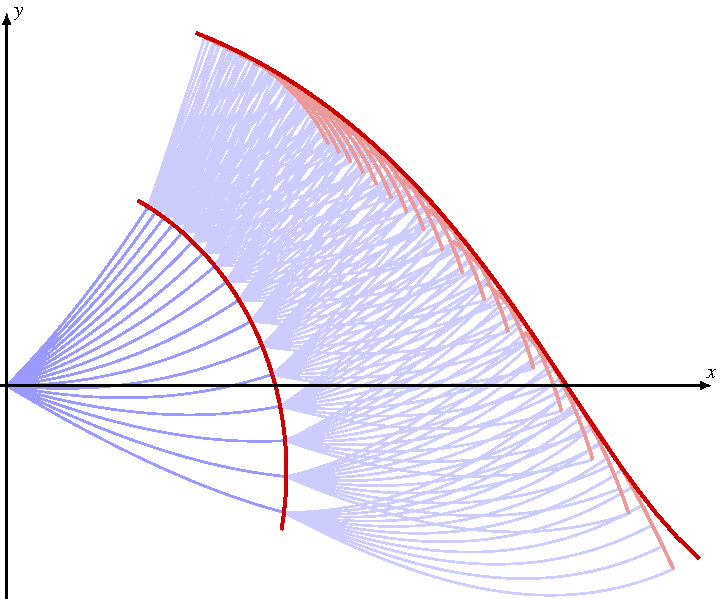
\includegraphics{chapters/080-hamiltonjacobi/examples/kreis.pdf}
\caption{Pseudokreise für das Funktional mit Lagrange-Funktion
$n(y)\sqrt{1+y^{\prime 2}}$.
Von den Punkten des ersten $J$-Kreises mit $J$-Radius 1 wird
jeweils ein weiterer Kreis mit Radius 1 gebildet.
Alle diese Kreise berühren den um den Nullpunkt gezogenen $J$-Kreis mit
Radius 2.
\label{buch:hamiltonjacobi:hamiltonjacobi:kreis}}
\end{figure}
